\section{}
\[
H(s)=\frac{s\,(0.1 - s)\,(s+10)}{(s+1)^2}\,.
\]
\subsection{Bode-Diagramm}
\begin{center}
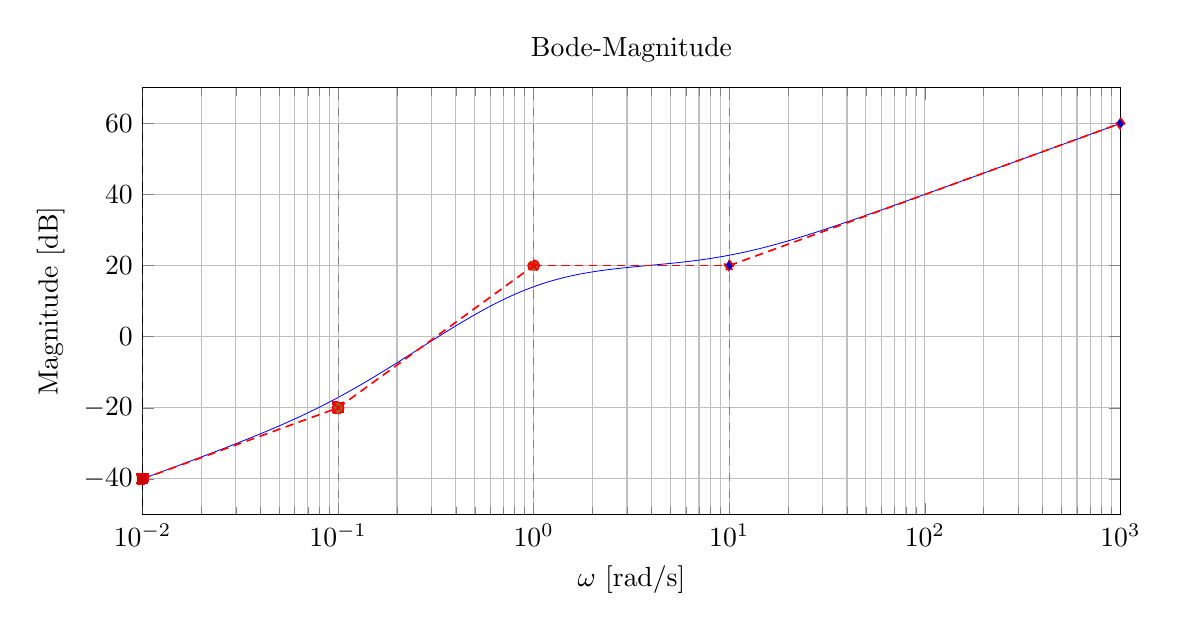
\begin{tikzpicture}
\begin{semilogxaxis}[
  width=14cm,height=7cm,
  ytick distance=20,
  xmin=1e-2,xmax=1e3,
  xlabel={$\omega$ [rad/s]},
  ylabel={Magnitude [dB]},
  grid=both,
  title={Bode-Magnitude}
]
\addplot[
  domain=1e-2:1e3,
  samples=800,
  mark=none,
  line width=0.3pt,
  blue
] {20*ln(x)/ln(10)
   +20*ln(sqrt(1 + (x/0.1)^2))/ln(10)
   +20*ln(sqrt(1 + (x/10)^2))/ln(10)
   -40*ln(sqrt(1 + x^2))/ln(10)};
\addplot+[domain=1e-2:1e-1,samples=2,dashed,dash pattern=on 3pt off 2pt,line width=0.6pt,red] {20*ln(x)/ln(10)};
\addplot+[domain=1e-1:1,samples=2,dashed,dash pattern=on 3pt off 2pt,line width=0.6pt,red] {40*ln(x)/ln(10) + 20};
\addplot+[domain=1:1e1,samples=2,dashed,dash pattern=on 3pt off 2pt,line width=0.6pt,red] {20};
\addplot+[domain=1e1:1e3,samples=2,dashed,dash pattern=on 3pt off 2pt,line width=0.6pt,red] {20 + 20*ln(x/10)/ln(10)};
\draw[gray,dashed] (rel axis cs:0,0) -- (rel axis cs:0,1);
\draw[gray,dashed] (axis cs:0.1,\pgfkeysvalueof{/pgfplots/ymin}) -- (axis cs:0.1,\pgfkeysvalueof{/pgfplots/ymax});
\draw[gray,dashed] (axis cs:1,\pgfkeysvalueof{/pgfplots/ymin}) -- (axis cs:1,\pgfkeysvalueof{/pgfplots/ymax});
\draw[gray,dashed] (axis cs:10,\pgfkeysvalueof{/pgfplots/ymin}) -- (axis cs:10,\pgfkeysvalueof{/pgfplots/ymax});
\node[gray,anchor=south east] at (axis cs:0.1,\pgfkeysvalueof{/pgfplots/ymax}) {\scriptsize Nullstelle $\omega_z=0.1$ (RHP)};
\node[gray,anchor=south east] at (axis cs:1,\pgfkeysvalueof{/pgfplots/ymax}) {\scriptsize Pol $\omega_p=1$ (doppelt)};
\node[gray,anchor=south east] at (axis cs:10,\pgfkeysvalueof{/pgfplots/ymax}) {\scriptsize Nullstelle $\omega_z=10$};
\end{semilogxaxis}
\end{tikzpicture}
\vspace{6mm}
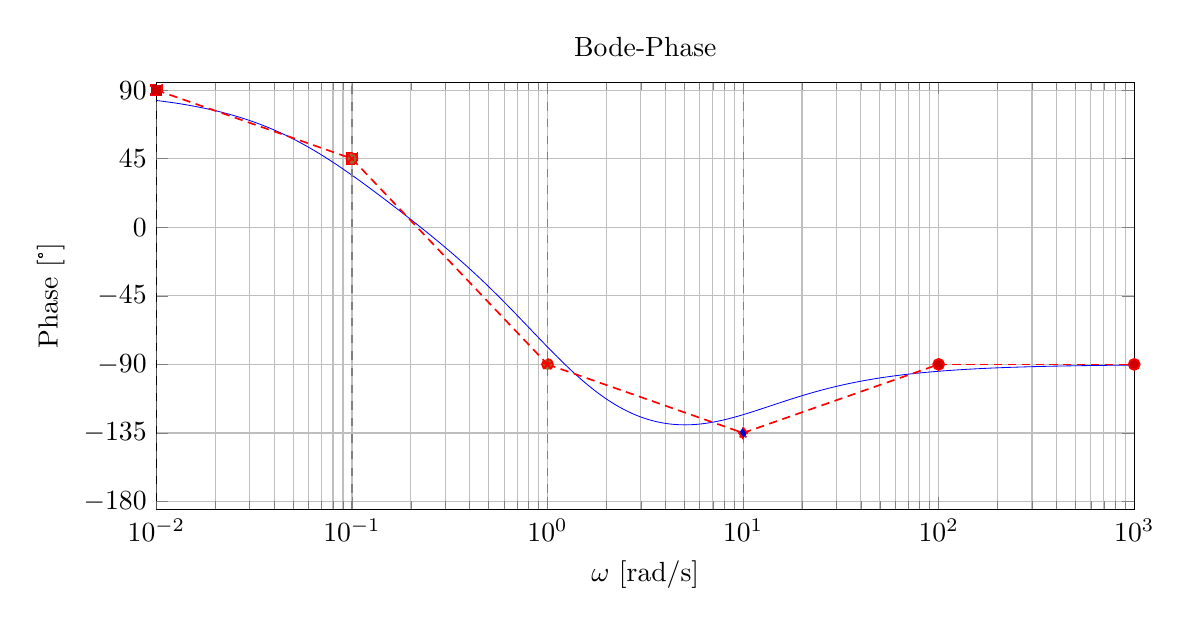
\begin{tikzpicture}
\begin{semilogxaxis}[
  width=14cm,height=7cm,
  xmin=1e-2,xmax=1e3,
  ytick distance=45,
  ymin=-185,ymax=95,
  xlabel={$\omega$ [rad/s]},
  ylabel={Phase [°]},
  grid=both,
  title={Bode-Phase}
]
\addplot[
  domain=1e-2:1e3,
  samples=800,
  mark=none,
  line width=0.3pt,
  blue
] {90 - atan(x/0.1) + atan(x/10) - 2*atan(x)};
\addplot+[domain=1e-2:1e-1,samples=2,dashed,dash pattern=on 3pt off 2pt,line width=0.6pt,red] {45 - 45*ln(x/0.1)/ln(10)};
\addplot+[domain=1e-1:1e0,samples=2,dashed,dash pattern=on 3pt off 2pt,line width=0.6pt,red] {45 - 135*ln(x/0.1)/ln(10)};
\addplot+[domain=1e0:1e1,samples=2,dashed,dash pattern=on 3pt off 2pt,line width=0.6pt,red] {-90 - 45*ln(x)/ln(10)};
\addplot+[domain=1e1:1e2,samples=2,dashed,dash pattern=on 3pt off 2pt,line width=0.6pt,red] {-135 + 45*ln(x/10)/ln(10)};
\addplot+[domain=1e2:1e3,samples=2,dashed,dash pattern=on 3pt off 2pt,line width=0.6pt,red] {-90};
\draw[gray,dashed] (rel axis cs:0,0) -- (rel axis cs:0,1);
\draw[gray,dashed] (axis cs:0.1,\pgfkeysvalueof{/pgfplots/ymin}) -- (axis cs:0.1,\pgfkeysvalueof{/pgfplots/ymax});
\draw[gray,dashed] (axis cs:1,\pgfkeysvalueof{/pgfplots/ymin}) -- (axis cs:1,\pgfkeysvalueof{/pgfplots/ymax});
\draw[gray,dashed] (axis cs:10,\pgfkeysvalueof{/pgfplots/ymin}) -- (axis cs:10,\pgfkeysvalueof{/pgfplots/ymax});
\node[gray,anchor=south east] at (axis cs:0.1,\pgfkeysvalueof{/pgfplots/ymax}) {\scriptsize Nullstelle $\omega_z=0.1$ (RHP)};
\node[gray,anchor=south east] at (axis cs:1,\pgfkeysvalueof{/pgfplots/ymax}) {\scriptsize Pol $\omega_p=1$ (doppelt)};
\node[gray,anchor=south east] at (axis cs:10,\pgfkeysvalueof{/pgfplots/ymax}) {\scriptsize Nullstelle $\omega_z=10$};
\end{semilogxaxis}
\end{tikzpicture}
\end{center}
\newpage

\subsection{Erklärung}
\begin{description}[leftmargin=1.2em,labelsep=.6em,font=\bfseries]

\item[1. Normalform herstellen.]
Bringe die Übertragungsfunktion in die Standardform.
\[
H(s)=K_0\cdot s^{\,r}\,(1-sT_{z1})\,(1+sT_{z2})\cdot\frac{1}{(1+sT_p)^2}
\]
mit
\[
K_0=1,\quad r=1,\quad T_{z1}=10,\quad T_{z2}=0.1,\quad T_p=1.
\]

\[\underline{F}_2(s)=(1-sT_{z1})\ \text{(RHP-Nullstelle)},\quad\]
\[\underline{F}_3(s)=(1+sT_{z2})\ \text{(LHP-Nullstelle)},\quad\]
\[\underline{F}_4(s)=\tfrac{1}{(1+sT_p)^2}\ \text{(Doppelpol)}.\]


\item[2. Eckfrequenzen bestimmen und sortieren.]
\[
\omega_{z1}=\frac{1}{T_{z1}}=0.1 \,\mathrm{rad/s}\,,\quad \omega_{p}=\frac{1}{T_{p}}=1\,\mathrm{rad/s}\,\ \text{(doppelt)},\quad \omega_{z2}=\frac{1}{T_{z2}}=10\,\mathrm{rad/s}\,\] 
\[\omega_{zR}<\omega_{p}<\omega_{zL}
\]

\item[3. Startpunkt des Amplitudengangs festlegen (Geradennäherung).]
Setze \(\omega_{\min}=\omega_{zR}=0.1\).
\[
F_{\mathrm{dB}}(\omega_{\min})=20\log_{10}\!\Big(|K_0F^*_{\mathrm{ges}}(0)|\,\omega_{\min}^{\,r}\Big)
=20\log_{10}(0.1)=-20\,\mathrm{dB}.
\]
Ankerpunkt: \(-20\,\mathrm{dB}\) bei \(\omega=0.1\).

\item[4. Verlauf links vom Startpunkt zeichnen.]
Für \(\omega<0.1\) Anfangssteigung \(r\cdot 20=+20\,\mathrm{dB/dec}\) \(\Rightarrow\) Gerade mit \(+20\,\mathrm{dB/dec}\) durch den Ankerpunkt.

\item[5. Steigungswechsel an den Eckfrequenzen eintragen.]
Nullstelle bei \(0.1\): \(+20\,\mathrm{dB/dec}\) \(\Rightarrow\) Netto \(+40\,\mathrm{dB/dec}\) in \([0.1,1]\).
Doppelpol bei \(1\): \(-40\,\mathrm{dB/dec}\) \(\Rightarrow\) Netto \(0\,\mathrm{dB/dec}\) in \([1,10]\).
Nullstelle bei \(10\): \(+20\,\mathrm{dB/dec}\) \(\Rightarrow\) Netto \(+20\,\mathrm{dB/dec}\) für \(\omega\gg10\).
Geradennäherung:
\[
|H(j\omega)|_{\mathrm{dB}}\approx
\begin{cases}
20\log_{10}\omega,& \omega\le 0.1,\\
40\log_{10}\omega+20,& 0.1<\omega\le 1,\\
20,& 1<\omega\le 10,\\
20+20\log_{10}(\omega/10),& \omega\ge 10.
\end{cases}
\]

\item[6. Eckabrundungen korrekt berücksichtigen.]
RHP-/LHP-Nullstelle: \(+3\,\mathrm{dB}\) am Knick (\(\omega=0.1\) bzw. \(10\)).
Doppelpol (\(\omega=1\)): \(-6\,\mathrm{dB}\) am Knick.

\item[7. Phasenstartwert festlegen.]
Da \(K_0\,F^*_{\mathrm{ges}}(0)>0\) und \(r=1\):
\[
\varphi(0)=0^\circ + r\cdot 90^\circ=+90^\circ.
\]

\item[8. Phasenänderung durch Nullstellen und Pol eintragen.]
Beiträge: RHP-Nullstelle \(-90^\circ\) über \([0.01,1]\); Doppelpol \(-180^\circ\) über \([0.1,10]\); LHP-Nullstelle \(+90^\circ\) über \([1,100]\).
Überlappungen addieren sich im jeweiligen Bereich (\([0.1,1]\) wirken RHP-Nullstelle und beide Pole gemeinsam; \([1,10]\) wirken beide Pole und die LHP-Nullstelle gemeinsam)).
Näherung:


\item[9. Grenzwerte und Konsistenz prüfen.]
DC: \(|H(0)|=0\Rightarrow -\infty\,\mathrm{dB}\), \(\varphi(0)=+90^\circ\).
HF: \(|H(j\omega)|\sim \omega\cdot \omega \cdot \omega / \omega^2=\omega \Rightarrow +\infty \,\mathrm{dB}\).
\end{description}

\subsubsection*{Stückweise Näherungen (für die Skizze)}
\[
|H(j\omega)|_{\mathrm{dB}}\approx
\begin{cases}
20\log_{10}\omega,& \omega\ll 0.1,\\[2pt]
40\log_{10}\omega+20,& 0.1\ll\omega\ll 1,\\[2pt]
20,& 1\ll\omega\ll 10,\\[2pt]
20+20\log_{10}(\omega/10),& \omega\gg 10,
\end{cases}
\]
\[
\varphi(\omega)\approx
\begin{cases}
+90^\circ,& \omega\le 0.01,\\[2pt]
45^\circ-45^\circ\log_{10}(\omega/0.1),& 0.01<\omega<0.1,\\[2pt]
45^\circ-135^\circ\log_{10}(\omega/0.1),& 0.1<\omega<1,\\[2pt]
-90^\circ-45^\circ\log_{10}\omega,& 1<\omega<10,\\[2pt]
-135^\circ+45^\circ\log_{10}(\omega/10),& 10<\omega<100,\\[2pt]
-90^\circ,& \omega\ge 100.
\end{cases}
\]

\newpage